\chapter{Résolution du système linéaire}

\paragraph{}
On s'intéresse dans ce chapitre à la résolution numérique d'un système linéaire $Ax = b$, de taille $N$.
On cherche donc $x\in\mathbb{K}^N$ avec le second membre $b\in\mathbb{K}^N$ et la matrice $A\in\matrixsymb{N}{K}$ connus.
Dans le cadre de l'énergétique et de la multi-physique, les équations sont réelles mais pour plus de généralité dans la suite on prend le corps $\mathbb{K} = \mathbb{R}\textrm{ ou }\mathbb{C}$.


\section{Contexte de résolution}

  \subsection{Système linéaire creux}

    \paragraph{}
		Comme cela a été mentionné, la taille des matrices rencontrées dans un problème typique de la simulation numérique de la dynamique des fluides est très grande.
		Les matrices ont également une autre propriété : la creusité.
		Puisque les matrices des systèmes linéaires à résoudre sont liées à une matrice jacobienne (voir équation (\ref{eq:linear})), un coefficient de la matrice symbolise une interaction entre deux points du maillage.
		On comprend alors que si le graphe de ces interactions dépend du schéma de discrétisation et d'intégration spatiale, deux points éloignés dans le maillage ne seront normalement pas reliés.
		Ainsi, les matrices présentent cette caractéristique notable qu'est la creusité et que l'on peut observer sur la figure \ref{fig:sparse}.
		On y voit en effet que la majorité des coefficients du système linéaire est 0.
		En pratique, les matrices rencontrées sont tellement grandes qu'il n'est pas possible de les stocker et de les utiliser sous leur forme dense.
		La propriété de creusité permettra d'utiliser des représentation astucieuses pour stocker les matrices en mémoire, telle que le format CSR (Compressed Sparse Row) \cite{Saad2003}.
		Ces formats permettent à la fois d'économiser de l'espace en mémoire lors du stockage de la matrice, mais également de réaliser des opérations telles que le produit matrice vecteur plus efficacement qu'avec une matrice dense de même taille.

		\begin{figure}
			\centering
			\begin{subfigure}[t]{0.3\textwidth}
				\centering
				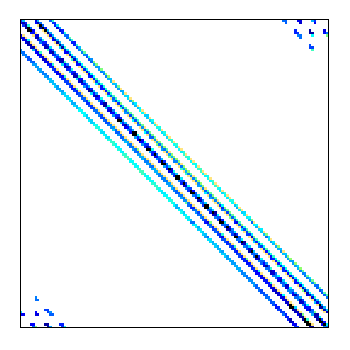
\includegraphics[width=\textwidth]{images/GT01R.png}
				\caption{GT01R : écoulement 2D non visqueux à travers un étage d'aubes de turbomachine}
				\label{fig:sparse.GT01R}
			\end{subfigure}
			\hfill
			\begin{subfigure}[t]{0.3\textwidth}
				\centering
				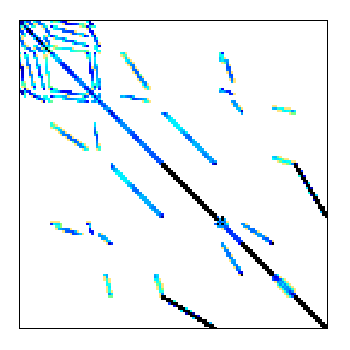
\includegraphics[width=\textwidth]{images/HV15R.png}
				\caption{HV15R : écoulement RANS 3D dans la soufflante d'un moteur}
				\label{fig:sparse.HV15R}
			\end{subfigure}
			\hfill
			\begin{subfigure}[t]{0.3\textwidth}
				\centering
				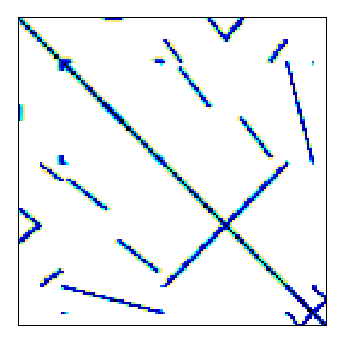
\includegraphics[width=\textwidth]{images/RM07R.png}
				\caption{RM07R : écoulement 3D visqueux dans le compresseur d'un turbopropulseur}
				\label{fig:sparse.RM07R}
			\end{subfigure}
			\caption{Représentation de matrices issues de problèmes de CFD \cite{PacullAubertBuisson2011}, utilisant une méthode spatiale Volumes Finis, les points de couleurs correspondant aux valeurs non nulles}
			\label{fig:sparse}
		\end{figure}


	\subsection{Type de méthode}

		\paragraph{}
		Il existe un grand nombre de méthodes pour inverser un problème linéaire.
		Cependant, en simulation numérique de la dynamique des fluides, la taille des maillage est souvent très importante (\PS{PAR EXEMPLE ?}), ce qui engendre des systèmes de très grande taille.
		Certaines méthodes de résolution ne sont alors plus compatibles, comme en particulier les méthodes directes.
		Cette famille de méthodes, dont fait partie par exemple la méthode du pivot de Gauss, calcule exactement la solution du système linéaire, mais nécessite un temps de calcul très important et un espace mémoire déraisonnable pour les tailles de nos problèmes.
		À l'inverse, les méthodes itératives produisent une suite de vecteurs qui convergent vers la solution du système linéaire.
		L'erreur sur la résolution du système décroît à mesure que l'algorithme itère et cela permet d'atteindre la précision souhaitée, non nulle mais suffisamment petite, pour un temps de calcul et une consommation mémoire maîtrisé.
		C'est l'idée que l'on retrouve sur la figure \ref{fig:direct-iterative} : la méthode directe ne fait aucun progrès avant $O\left(N^3\right)$ opérations, alors que la norme de l'erreur décroît avec le numéro d'itération pour la méthode itérative.

		\begin{figure}
			\centering
			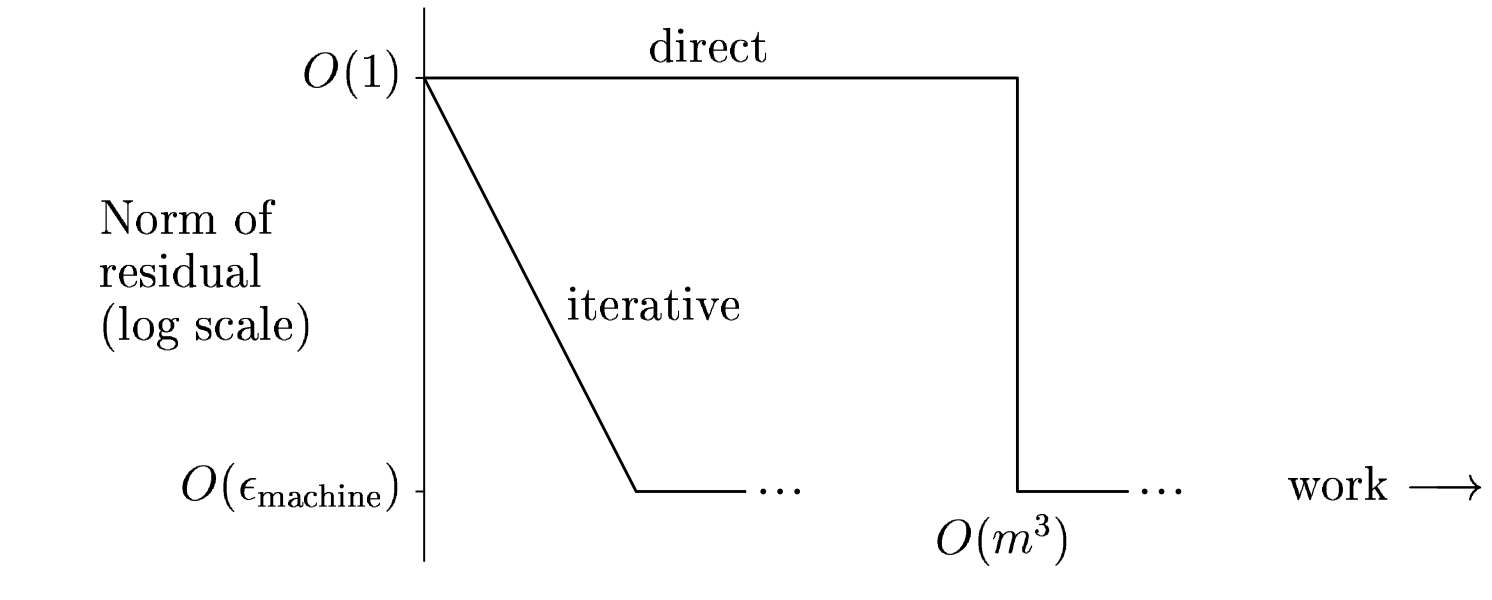
\includegraphics[width=.7\textwidth]{images/direct-iterative.png}
			\caption{Convergence des méthodes directes et itératives, issu de \cite{TrefethenBau1997}}
			\label{fig:direct-iterative}
		\end{figure}

		\paragraph{}
		Les méthodes itératives sont donc les plus adaptées pour inverser des systèmes linéaires creux de grande taille.
		Cependant, il peut arriver qu'on utilise une méthode directe : on peut envisager par exemple la résolution d'un système linéaire avec une succession d'étages d'un algorithme multigrille, pour arriver à un système grossier de petite taille (ou au moins de taille raisonnable), qu'on résoudrait avec une méthode directe comme la décomposition LU.
		Ces méthodes sont bien connues \cite{TrefethenBau1997}, et ne seront pas détaillées ici.


	\subsection{Méthodes itératives}

		\paragraph{}
		Les méthodes itératives sont encore aujourd'hui très étudiées dans la communauté des mathématiques appliquées \cite{OlshanskiiTyrtyshnikov2014, Saad2003, TrefethenBau1997}.
		Une première classe de méthode intervient : les méthodes itératives classiques.
		Ce sont des méthodes de relaxation, parmi lesquelles on compte les méthode de Jacobi, Gauss-Seidel ou encore SOR (Successive Over Relaxation).
		Leur fonctionnement réside dans une décomposition $A = M - N$ avec $M$ une matrice relativement facile à inverser, où le choix de la décomposition est propre à la méthode.
		Pour la méthode de Jacobi on prendra pour $M$ la diagonale de $A$.
		Il suffit ensuite, à partir d'un itéré initial $x_0$ d'appliquer la formule de récurrence $x_{n+1} = M^{-1}\left(Nx_n + b\right)$.
		Cependant, comme dit précédemment, ces méthodes n'offrent pas une convergence satisfaisante pour la communauté de CFD.
		Ainsi, il faut se tourner vers un autre type de méthodes itératives pour résoudre le système linéaire.

		\paragraph{}
		Si ces méthodes sont plutôt anciennes et plutôt écartées pour leurs mauvaises performances, elles peuvent s'utiliser en se combinant avec des 	méthodes plus efficaces, et c'est pour cela qu'il est important de comprendre leur fonctionnement.
		En particulier, la méthode de Jacobi est toujours utilisée, car si elle est plutôt simple et offre une convergence plutôt lente, elle est très peu coûteuse et se parallélise facilement, ce qui est un argument de poids lorsqu'on traite des systèmes de très grande taille.


\section{Méthodes de Krylov}

  \subsection{Principe des méthodes}

    \paragraph{}
    Les méthodes de Krylov s'imposent comme étant la norme dans le domaine de la dynamique des fluides numérique.
    \footnote{\GP{Qui l'a dit? Ou as-tu trouve la reference?}\PS{Je voulais dire par là que de ce que j'ai vu, beaucoup de monde les utilise. Personne n'a explicitement dit ça, est ce que je remplace par : Les méthodes de Krylov semblent s'imposer dans le domaine de la dynamique des fluides.}}
    Le principe d'une méthode de Krylov est de projeter le système linéaire sur un espace restreint appelé espace de Krylov, et d'y résoudre le système maintenant qu'il est plus petit.
		L'astuce va être dans le fait que ces espaces de Krylov sont emboîtés, et qu'a chaque nouvelle itération on utilise l'information accumulée lors des précédentes.

		\paragraph{}
		Dans ce qui suit, on notera à l'itération $n$ le résidu $r_n = b - Ax_n$, où $x_n$ est l'itéré produit par l'algorithme.
		Dans la pratique, on se restreint à un nombre d'itérations $n\ll N$ pour des raisons évoquées précédemment, mais la suite reste vraie pour $n\le N$.
		On supposera également que l'équation (\ref{eq:linear}) admet une solution.
		Enfin, on notera que résoudre $Ax = b$ avec un itéré initial $x_0$ est équivalent ici à résoudre $A\tilde{x} = b - Ax_0$ avec un itéré initial nul, puis à prendre $x_0 + \tilde{x}$ comme vecteur solution.

		\paragraph{}
		Pour résoudre $Ax = b$ en partant d'un itéré initial $x_0$ et donc d'un résidu $r_0 = b - Ax_0$, on définit l'espace de Krylov à l'itération $n$:
		\begin{equation}\label{eqn:krylov}
			\krylov[A, r_0]{n} = \operatorname{Vect}\left(r_0, Ar_0, \dots, A^{n-1}r_0\right)\ .
		\end{equation}
		On constate alors que par définition $\krylov{1}\subset\krylov{2}\subset\dots\subset\krylov{n-1}\subset\krylov{n}$.
		On cherche ensuite l'itéré sur $\krylov{n}$ qui garantit une condition de Petrov-Galerkin \cite{SimonciniSzyld2007} :
		\begin{equation}\label{eqn:x_n}
			x_n \in x_0 + \krylov[A, r_0]{n}\quad\textrm{tel que}\quad x_n \perp \mathcal{L}_n
		\end{equation}
		où $\mathcal{L}_n$ est un sous-espace vectoriel de dimension $n$.
		Pour $\mathcal{L}_n = \krylov{n}$ on parle de condition de Galerkin, et pour $\mathcal{L}_n = A\krylov{n}$ de minimisation du résidu.
		On voit donc que si $A$ est inversible, $\mathcal{L}_N = \mathbb{K}^N$ et alors l'algorithme termine en au plus $N$ itérations.
		Cette remarque n'a pas grand intérêt en pratique puisqu'on arrêtera l'algorithme bien avant.

		\paragraph{}
		Pour construire les différents espaces de Krylov, on utilise l'itération d'Arnoldi \cite{TrefethenBau1997}.
		La matrice $A$ est semblable à une matrice de Hessenberg $H$ :
		\begin{equation}\label{eq:hessenberg}
			A = VH\adj{V}\Leftrightarrow AV = VH\quad\textrm{avec}\quad H=
			\begin{pmatrix}
				h_{1,1}&h_{1,2}&h_{1,3}&\cdots &h_{1,N}\\
				h_{2,1}&h_{2,2}&h_{2,3}&\cdots &h_{2,N}\\
				0      &h_{3,2}&h_{3,3}&\cdots &h_{3,N}\\
				\vdots &\ddots &\ddots &\ddots &\vdots \\
				0      &\cdots &0      &h_{N,N-1}&h_{N,N}
			\end{pmatrix}\ .
		\end{equation}
		Dans (\ref{eq:hessenberg}), $V$ est une matrice orthonormale de taille $N$.
		On notera $v_i$ sa $i^{\textrm{ème}}$ colonne.
		On notera également $V_n\in\matrixsymb{N, n}{K}$ la matrice constituée des $n$ premières colonnes de $V$.
		On notera enfin $\widetilde{H}_n\in\matrixsymb{n+1, n}{K}$ le bloc supérieur gauche de $H$, qui est également de Hessenberg.

		\paragraph{}
		En considérant les $n \le N$ premières colonnes de (\ref{eq:hessenberg}), de par la structure de Hessenberg de $H$, on obtient la relation d'Arnoldi :
		\begin{equation}\label{eq:arnoldi}
			AV_n = V_{n+1}\widetilde{H}_n
		\end{equation}
		et en considérant la dernière colonne de l'équation (\ref{eq:arnoldi}) :
		\begin{equation}\label{eq:arnoldi_n+1}
			Av_n = h_{1,n}v_1 + \dots + h_{n,n}v_n + h_{n+1,n}v_{n+1}\ .
		\end{equation}

		\paragraph{}
		On peut maintenant décrire l'algorithme :
		Puisque $\krylov{1} = \operatorname{Vect}\left(r_0\right)$, on pose $v_1 = \frac{r_0}{\norm{r_0}}$.
		On itère ensuite sur $n$ : en connaissant $V_n$, la relation (\ref{eq:arnoldi_n+1}) permet de trouver le nouveau vecteur de base et la $n$\textsuperscript{ième} colonne de $H$, c'est à dire de trouver $V_{n+1}$ et $\widetilde{H}_n$.
		Les espaces vectoriels $\operatorname{Im}\left(V_n\right)$ sont alors par construction les espaces de Krylov $\krylov{n}$.

		\paragraph{}
		On remarque que la matrice $A$ n'intervient dans la relation (\ref{eq:arnoldi_n+1}) qu'à travers le produit $Av_n$.
		Il n'est donc pas nécessaire de former explicitement la matrice du système linéaire, mais seulement de pouvoir calculer son action sur un vecteur.
		Cette propriété des méthodes de Krylov sera utilisée par la suite.

		\paragraph{}
		Il existe donc beaucoup de méthodes de Krylov pour résoudre un système linéaire, la principale distinction entre elle se faisant par le choix du sous-espace $\mathcal{L}_n$.
		La condition de minimisation du résidu donne la méthode GMRES, qui est l'une des plus utilisée par les communautés de CFD et de mathématiques appliquées.
		Elle permet, après des itérations un peu plus coûteuses que ses consœurs telles que la méthode Bi-CG \cite{TrefethenBau1997}, de minimiser le résidu obtenu et donc de garantir la décroissance de l'erreur.
		De plus, la méthode GMRES est beaucoup étudiée et de nombreuses variantes et améliorations ont été développées au fil des années.
		Pour ces raisons, et parce que son implémentation est relativement simple, c'est sur cette méthode que j'ai décidé de m'orienter.


	\subsection{GMRES}

		\paragraph{}
		La méthode GMRES \cite{SaadSchultz1986} consiste donc, à chaque itération $n$, à :
		\begin{itemize}
			\item calculer le nouvel espace de Krylov $\krylov{n+1}$ à partir de $\krylov{n}$, donc d'après (\ref{eq:arnoldi_n+1}) de calculer le produit $Av_n$, puis de l'orthonormaliser sur les colonnes de $V_n$ pour obtenir $\widetilde{H}_n$ et $V_{n+1}$
			\item trouver $x_n \in x_0 + \krylov{n}$ qui minimise la norme de $r_n = b - Ax_n$.
		\end{itemize}
		Puisque $x_n \in x_0 + \krylov{n}$, $x_n = x_0 + V_n y_n$ pour un certain $y_n\in\mathbb{K}^n$.
		On dispose de la relation d'Arnoldi (\ref{eq:arnoldi}), donc :
		\begin{align*}
			\norm{r_n} &= \norm{b - Ax_n} \\
			&= \norm{r_0 - AV_ny_n} \\
			&= \norm{r_0 - V_{n+1}\widetilde{H}_ny_n} \\
			&= \norm{\norm{r_0} e_1 - \widetilde{H}_ny_n}\qquad\textrm{avec $e_1$ le premier vecteur de la base canonique de $\mathbb{K}^{n+1}$.}
		\end{align*}

		\paragraph{}
		La condition de minimisation du résidu est remplie en résolvant un problème de minimisation de taille $n$.
		En pratique ce problème est résolu par décomposition QR de la matrice de Hessenberg.
		Pour ce faire, on suppose qu'on dispose d'une décomposition $\Omega_n\widetilde{H}_n = \begin{pmatrix}R_n \\ 0\end{pmatrix}$ avec $\Omega_n\in\orthogroup{n+1}{K}$ une matrice unitaire et $R_n\in\matrixsymb{n}{K}$ une matrice diagonale.
		La décomposition QR de $\widetilde{H}_n$ à en effet cette forme de par sa structure de Hessenberg.
		C'est le cas à l'itération 1 avec $\Omega_1 = \operatorname{Id}$ et $R_1 = 1$.
		On note ensuite :
		\[\begin{pmatrix}\Omega_n & 0 \\ 0 & 1\end{pmatrix}\widetilde{H}_{n+1} = \begin{pmatrix}R_n & r_{n+1} \\ 0 & \rho \\ 0 & \sigma\end{pmatrix} \quad\textrm{avec}\quad \begin{pmatrix}r_{n+1} \\ \rho\end{pmatrix} = \Omega_n\begin{pmatrix}h_{n,n+1} \\ \vdots \\ h_{n+1,n+1}\end{pmatrix} \quad\textrm{et}\quad \sigma = h_{n+2,n+1}\ .\]
		On pose ensuite la rotation de Givens :
		\[G_n = \left\{\begin{aligned}
			&\quad\operatorname{Id}_{n+2} &\textrm{si }\rho = \sigma = 0\\ \\
			\begin{pmatrix}\operatorname{Id}_n & 0 & 0 \\ 0 & c & s \\ 0 & -s & c\end{pmatrix}& \quad\textrm{avec}\quad c = \frac{\rho}{\sqrt{\rho^2 + \sigma^2}}, s = \frac{\sigma}{\sqrt{\rho^2 + \sigma^2}} &\quad\textrm{sinon.}
		\end{aligned}\right.\]
		On remarque enfin que :
		\[G_n\begin{pmatrix}\Omega_n & 0 \\ 0 & 1\end{pmatrix}\widetilde{H}_{n+1} = \begin{pmatrix}R_n & r_{n+1} \\ 0 & \sqrt{\rho^2 + \sigma^2} \\ 0 & 0\end{pmatrix}\]
		ce qui donne la nouvelle décomposition QR : $\Omega_{n+1}\widetilde{H}_{n+1} = \begin{pmatrix}R_{n+1} \\ 0\end{pmatrix}$.


		\paragraph{}
		Finalement, la décomposition QR de la matrice de Hessenberg se construit à mesure des itérations, de manière peu coûteuse.
		Cette décomposition est cependant très intéressante.
		Lorsqu'on cherche à minimiser le résidu, on à montré précédemment qu'on minimise :
		\begin{align*}
			\norm{r_n} &= \norm{\norm{r_0} e_1 - \widetilde{H}_ny_n} \\
			&= \norm{\norm{r_0} \Omega_ne_1 - \begin{pmatrix}R_ny_n \\ 0\end{pmatrix}}\ .
		\end{align*}
		La solution de ce problème de minimisation est connu.
		En notant $\Omega_ne_1 = \begin{pmatrix}\omega_1 \\ \omega_{1n}\end{pmatrix}$ la première colonne de $\Omega_n$, on a :
		\[y_n = \norm{r_0}R_n^{-1}\omega_1\quad\textrm{et}\quad\norm{r_n} = \norm{r_0}\left|\omega_{1n}\right|\ .\]
		L'intérêt de mettre à jour la décomposition de la matrice de Hessenberg est alors double :
		\begin{itemize}
			\item l'inversion du système réduit est explicite, par inversion d'une matrice triangulaire ce qui est aisé
			\item la norme du résidu peut être calculée à chaque itération sans inverser le système, ce qui permet un meilleur contrôle des itérations.
		\end{itemize}

		\paragraph{}
		Mon choix s'est porté sur la méthode GMRES pour plusieurs raisons.
		Tout d'abord, c'est une méthode de Krylov, et le choix de ce type de méthode a déjà été argumenté précédemment.
		Ensuite, cette méthode permet un contrôle du résidu, car la norme de celui ci décroît entre chaque itération.
		Ce n'est pas le cas pour toutes les méthodes de Krylov comme par exemple pour la méthode Bi-CG.
		GMRES est un algorithme relativement simple qui ne nécessite pas (ou peu) de réglages, que ce soit de la part du développeur ou bien de l'utilisateur.
		Cette méthode de résolution du système linéaire est encore aujourd'hui bien présente au sein de la communauté de mathématiques appliquées \cite{Vasseur2016}, de CFD \cite{FrancoCamierAndrejEtAl2020} et est utilisée dans bien d'autres domaines, comme par exemple l'électromagnétisme \cite{ErnstGander2012} ou la mécanique du solide \cite{Mercier2015}.


	\subsection{Convergence des méthodes}

		\paragraph{}
		La convergence des méthodes de Krylov, et plus généralement des méthodes itératives, dépend du système linéaire.
		En effet, si une méthode itérative fait converger la norme de l'erreur ou celle du résidu vers 0, la vitesse de convergence dépend à la fois de la méthode et de la matrice à inverser.

		\paragraph{}
		On se rend compte en parcourant la littérature \cite{Nevanlinna1994} que la convergence des méthode itératives est très fortement liée au conditionnement de l'opérateur $A$.
		Le conditionnement d'une matrice inversible $A$ est :
		\[\kappa\left(A\right) = \norm{A}\norm{A^{-1}}\]
		et dépend donc de la norme choisie.
		Une matrice dite bien conditionnée, du point de vue des algorithmes itératifs, a un conditionnement $\kappa = O\left(1\right)$.
		Au contraire, pour une matrice mal conditionnée, $\kappa\gg1$.

		\paragraph{}
		Pour la norme $\norm[2]{\cdot}$ on a, pour une matrice $A$ :
		\begin{equation}\label{eq:conditionnement}
			\kappa\left(A\right) = \frac{\sigma_{\max}}{\sigma_{\min}}
		\end{equation}
		où $\sigma_{\min}$ et $\sigma_{\max}$ sont les valeurs singulières minimales et maximales de $A$.
		Pour rappel, les valeurs singulières de $A$ sont les valeurs propres de $\adj{A}A$.

		\paragraph{}
		On trouve souvent la relation : $\kappa\left(A\right) = \frac{\left|\lambda_{\max}\right|}{\left|\lambda_{\min}\right|}$ avec $\lambda_{\min}$ et $\lambda_{\max}$ les valeurs propres de $A$ de plus petit et de plus grand module.
		Cependant cette relation n'est vraie que pour les matrices normales (qui commutent avec leur matrice adjointe).
		Pour cette raison, il ne sert à rien de se baser uniquement sur le spectre de l'opérateur pour étudier la convergence des méthodes.

		\paragraph{}
		Dans \cite{GreenbaumPtakStrakos1996}, on trouve un résultat surprenant.
		Cet article montre en effet que pour un spectre donné et pour une courbe de convergence décroissante donnée, il est possible de construire une matrice avec ce spectre telle que GMRES suivra la courbe de convergence.
		Autrement dit, on peut exhiber un exemple de matrice mal conditionnée qui converge rapidement, et à l'inverse trouver une matrice bien conditionnée pour laquelle GMRES aura du mal à faire décroitre le résidu.
		En particulier, on peut concevoir une matrice avec le meilleur spectre possible, c'est à dire qui admet 1 comme seule valeur propre de multiplicité $N$, et pour qui GMRES convergerait aussi lentement que souhaité.
		Ce phénomène est causé par la non-normalité de l'opérateur \cite{GreenbaumStrakos1994, GreenbaumPtakStrakos1996}.
		Pour remédier à ce problème, on peut par exemple s'intéresser au pseudo-spectre de l'opérateur \cite{Trefethen1999}.
		Cependant, cette analyse est relativement complexe et ne sera pas présentée ici.

		\paragraph{}
		L'utilisation des méthodes de Krylov avec ces matrices non-normales, et l'analyse de la convergence des algorithmes pour ces matrice ne sont pas triviales \cite{LiesenTichy2004, Huhtanen2005}.
		Puisque les matrices rencontrées dans les problèmes de CFD sont quelconques, ou au moins à priori non-normales, étudier précisément le spectre de l'opérateur ne semble pas être une bonne idée.

		\paragraph{}
		Si une étude précise du spectre de la matrice n'est pas recomandée, une rapide analyse peut toutefois s'avérer utile.
		En effet, mathématiquement parlant, le spectre peut ne donner aucune information, d'après le paragraphe précédent.
		Cependant, les matrices rencontrées en pratiques ne sont pas des contres-exemples d'une preuve mathématique, mais de vraies matrices quelconque.
		En faisant l'hypothèse qu'on ne tombera pas précisément sur un cas particulier, on peut continuer à regarder le spectre de $A$ pour se donner une idée de la convergence de l'algorithme.

		\subsubsection{Convergence de GMRES}

			\paragraph{}
			Pour étudier la convergence de GMRES, on reformule le problème de minimisation \cite{TrefethenBau1997}.
			On prendra dans ce qui suit une norme quelconque de $\mathbb{K}^n$ et sa norme induite pour $\matrixsymb{n}{K}$.
			Pour $x_n\in\krylov{n}$, on peut écrire $x_n = x_0 + q_n\left(A\right)b$ où $q_n\left(X\right)$ est un polynôme de $\mathbb{K}_{n-1}\left[X\right]$.
			Le résidu devient alors $r_n = b - Ax_n = p_n\left(A\right)r_0$ où $p_n\left(X\right)\in\mathbb{K}_n\left[X\right]$ s'écrit $p_n\left(X\right) = 1 - Xq_n\left(X\right)$.
			En notant $\textup{P}_n = \left\{\,p\in\mathbb{K}_n\left[X\right]\;\mid\;p\left(0\right) = 1\,\right\}$, le problème de minimisation devient alors :
			\[\textrm{trouver $p_n\in \textup{P}_n$ qui minimise $\norm{p_n\left(A\right)r_0}$.}\]


			\paragraph{}
			Nous avons déjà dit que pour GMRES, $\norm{r_{n+1}}\leq\norm{r_n}$, et que $\norm{r_N} = 0$.
			En utilisant le résultat du paragraphe précédent, on a de plus que $\norm{r_n} = \norm{p_n\left(A\right)r_0}\leq\norm{p_n\left(A\right)}\norm{r_0}$. Ainsi :
			\[\frac{\norm{r_n}}{\norm{r_0}} \leq \inf_{p\in\textup{P}_n}\norm{p\left(A\right)}\ .\]

			\paragraph{}
			Supposons maintenant que $A$ est diagonalisable, avec $A = VDV^{-1}$ pour une matrice inversible $V$ et une matrice diagonale $D$.
			La diagonale de $D$ est en fait composée des valeurs propres de $A$ : $\lambda_1, \dots, \lambda_N$.
			Alors pour un polynôme $p$ on a $\norm{p\left(A\right)}\leq\norm{V}\norm{p\left(D\right)}\norm{V^{-1}}$
			Ainsi, on a la relation :
			\[\frac{\norm{r_n}}{\norm{r_0}} \leq \kappa\left(V\right)\inf_{p\in\textup{P}_n}\max_{1\leq i\leq N}\norm{p\left(\lambda_i\right)}\ .\]
			On comprend alors la remarque faite précédemment : si la matrice $A$ n'est pas trop non-normale, c'est à dire si $\kappa\left(V\right)$ n'est pas trop grand, alors la convergence de GMRES est controlée par les valeurs propres de $A$.


\section{Améliorations de l’algorithme}

	\paragraph{}
	Dans la suite on suppose qu'on dispose d'une méthode de résolution du problème linéaire (\ref{eq:linear}).
	Conformément à ce qui a été argumenté dans les parties précédentes, on prendra donc une méthode de Krylov : la méthode GMRES.
	Nous pouvons déjà appliquer cette méthode pour obtenir une solution au système linéaire, cependant il est possible de faire mieux.
	En effet, la méthode GMRES peut être améliorée, affinée, pour obtenir plus efficacement la solution.
	De telles améliorations sont présentées dans ce qui suit.
	Il sera précisé si cette amélioration concerne typiquement la méthode GMRES, ou si elle s'applique généralement à toute méthode de résolution d'un système linéaire.


	\subsection{Préconditionnement}

		\paragraph{}
		Nous avons expliqué précedemment en quoi le conditionnement de l'opérateur linéaire joue sur la vitesse de convergence des algorithmes itératifs.
		On peut utiliser un préconditionnement pour jouer sur le spectre de la matrice afin d'améliorer son conditionnement.
		Un préconditionnement, ou préconditionneur, est associé à une matrice $M$.
		Le principe est de multiplier l'équation à résoudre par cette matrice, pour modifier l'opérateur à inverser.
		Concrètement, on peut effectuer un préconditionnement à gauche :
		\[M^{-1}Ax = M^{-1}b\]
		ou bien un préconditionnement à droite :
		\[\left\{\begin{aligned}AM^{-1}x' &= b \\	M^{-1}x' &= x\end{aligned}\right.\ .\]
		Pour un préconditionnement à gauche, respectivement à droite, l'opérateur à inverser est alors $M^{-1}A$, respectivement $AM^{-1}$.
    On notera qu'avec un préconditionneur à droite appliqué à une méthode de Krylov, la relation d'arnoldi (\ref{eq:arnoldi}) devient :
    \begin{equation}\label{eq:arnoldi_pre}
      AM^{-1}V_n = V_{n+1}\widetilde{H}_n\ .
    \end{equation}

		\paragraph{}
		L'idée principale du préconditionnement est de transformer $A$ en une matrice plus facile à inverser.
		On prend donc pour $M$ une matrice qui ressemble à $A$.
		Si $M$ est trop proche de $A$, par exemple $M=A$, l'équation préconditionnée devient triviale.
		Cependant appliquer le préconditionnement, c'est à dire calculer $M^{-1}$ est aussi dur que de résoudre le problème initial.
		À l'inverse, si on prend un préconditionneur facile à inverser mais trop éloigné de $A$, typiquement $M = \operatorname{Id}$, alors le calcul du préconditionnement est trivial, mais il n'aide pas à résoudre le problème.
		On va donc faire un compromis pour trouver un opérateur $M$ qui ressemble à $A$, mais qu'il est relativement facile d'inverser.

		\paragraph{}
		En s'inspirant de l'exemple 35.2 de \cite{TrefethenBau1997}, on considère la matrice complexe de taille $N\times N$ avec $N = 200$ qui est la somme d'une matrice diagonale et d'une matrice de perturbations aléatoires :
		\[A = A_{diag} + \frac{1}{2\sqrt{N}}A_{rand}\]
		où
		\[A_{diag, k} = 2\sin\left(\frac{2k\pi}{N-1}\right) - 1 + i\cos\left(\frac{2k\pi}{N-1}\right) \quad\textrm{et}\quad A_{rand}\hookrightarrow\mathcal{N}\left(0,1\right)\ .\]

		\paragraph{}
		On représente sur la figure \ref{fig:precond} le spectre de $A$ en bleu.
		On y voit qu'il est étalé tout autour de l'origine.
		En appliquant un préconditionneur de Jacobi, détaillé par la suite, on voit que le spectre préconditionné est rassemblé autour de 1.
		L'effet du préconditionneur sur la convergence de GMRES se voit très nettement sur la figure.
		Pour la matrice non préconditionnée, les itérations peinent à faire décroitre la norme du résidu, alors que celle-ci chute rapidement lorsqu'on applique le préconditionneur.

		\paragraph{}
		Cet exemple permet également d'établir une remarque intéressante.
		En effet, déjà avant de préconditionner la matrice, son conditionnement n'est pas excessivement grand, et cependant GMRES n'arrive pas à converger.
		C'est parce que puisque la matrice est non-normale, le conditionnement seul ne veut rien dire, et dans cet exemple en particulier c'est la disposition des valeurs propres qui importent.
		Ainsi, l'étude du spectre de l'opérateur ne peut se faire en regardant simplement son conditionnement.
		Il faut aussi regarder la répartition de ses valeurs propres dans le plan complexe, sa non-normalité, ...

		\begin{figure}
			\centering
			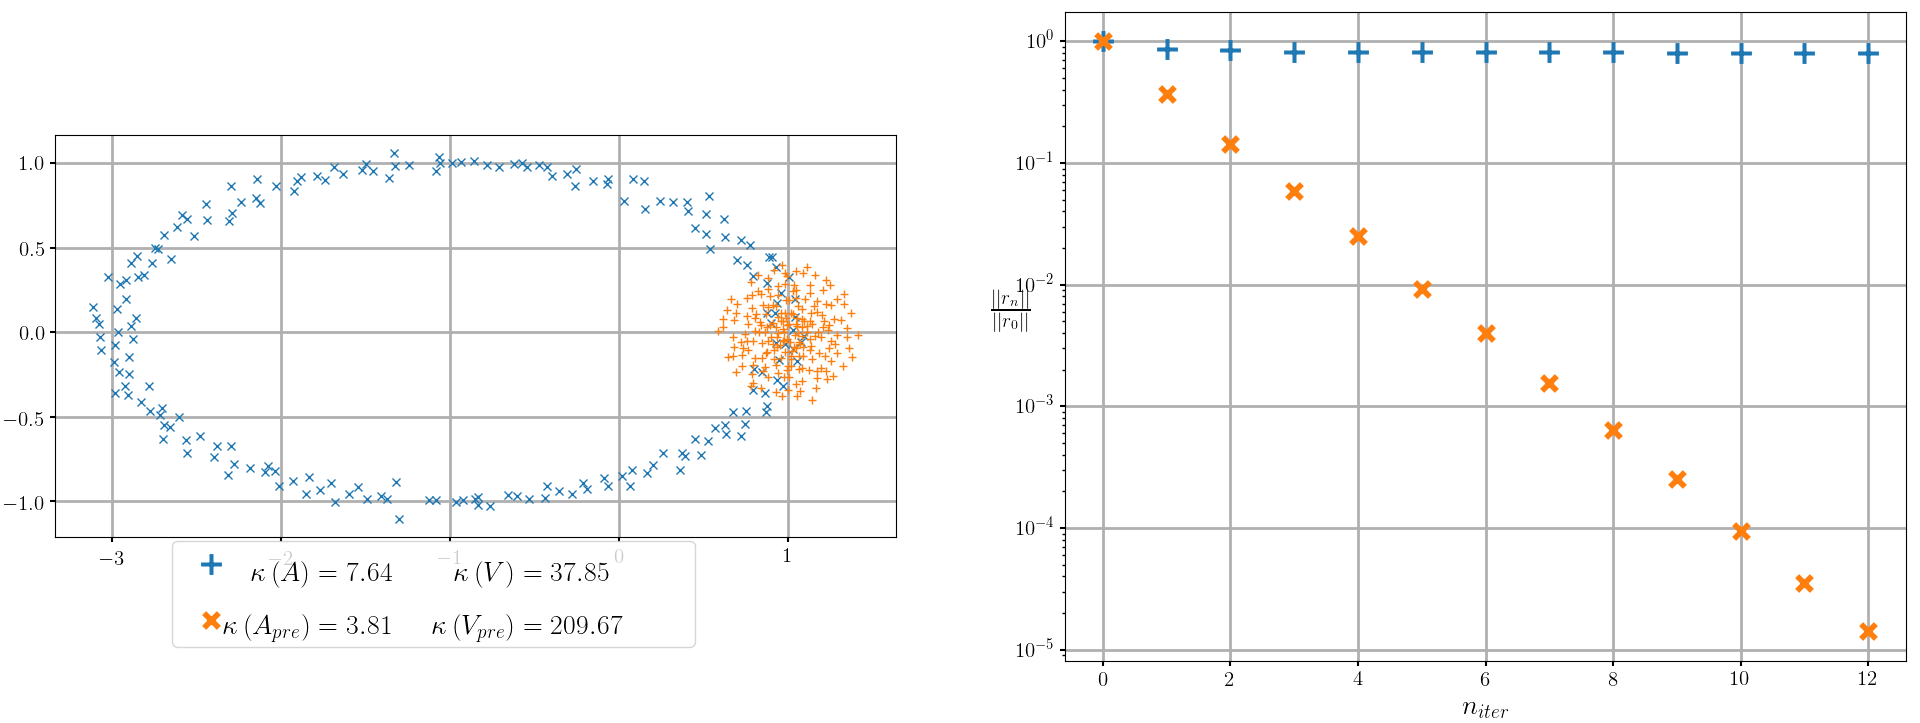
\includegraphics[width=\textwidth]{images/precond.png}
			\caption{Spectre de $A = VDV^{-1}$ en bleu et de $A_{pre} = AD^{-1}$ en orange (gauche). Convergence de GMRES pour ces matrices (droite).}
			\label{fig:precond}
		\end{figure}


		\paragraph{}
		Ci après sont brièvement présentés les préconditionnements les plus connus, qui s'appliquent de manière générale à toute méthode de résolution d'un système linéaire.


		\paragraph{Préconditionneur de Jacobi :}
		aussi appelé préconditionneur Diagonal, on prend $M=\operatorname{diag}\left(A\right)$, à condition qu'il n'y ait pas de zéros sur la diagonale de $A$.
		De manière plus générale, on peut prendre $M$ comme matrice diagonale telle que le conditionnement de $M^{-1}A$ est meilleur que celui de $A$.
		Ce préconditionneur est très intéressant pour les matrices à diagonale dominante.
		Dans ce cas, le théorème de Gerschgorin garantit l'efficacité d'un tel préconditionneur.
		Dans le cas plus général, il est souvent insuffisant.
		Ce préconditionneur est de plus facile à mettre en place, nécessite peu d'espace mémoire et est peu coûteux à calculer.
		S'il est très basique, il s'avère être très souvent employé grâce à sa grande simplicité et a ses bonnes performances pour le calcul parallèle.

		\paragraph{Approximation Locale :}
		quand $A$ représente un couplage entre deux échelles, phénomènes physiques, ..., on prend pour $M$ le même opérateur mais sans les termes d'interaction.
		Cela consiste à garder quelques éléments proches de la diagonale, et à généraliser le préconditionneur de Jacobi.
		Un cas particulier est le préconditionneur diagonal par bloc, qui consiste à garder les blocs diagonaux représentants différents domaines, mais de supprimer les blocs extra-diagonaux représentant les interactions entre domaines.
		L'avantage de ces préconditionneurs est à nouveau qu'ils sont naturellement parallélisables.

		\paragraph{Factorisation incomplète :}
		quand on dispose d'une factorisation de $A$ et que la matrice $A$ est creuse, les matrices intervenant dans ces décomposition perdent la creusité.
		On va donc garder ces matrices en leur imposant le pattern de creusité de $A$.
    Par exemple, pour une décomposition LU, $A = LU$ avec $L$ et $U$ des matrices triangulaire, respectivement inférieure et supérieure.
		On prend alors $M=\widetilde{L}\widetilde{U}$ avec $\widetilde{L}_{ij}=L_{ij}$ et $\widetilde{U}_{ij}=U_{ij}$ si $A_{ij}\neq0$ et $\widetilde{L}_{ij}=\widetilde{U}_{ij}=0$ sinon.
    On appelle cette factorisation ILU, ou ILU(0).
		On peut généraliser cette factorisation incomplète en prenant le pattern de creusité de $A^{k+1}$, plus dense que le pattern de creusité de $A$ mais globalement creux.
    On parle alors de factorisation ILU($k$).
		Cette famille de préconditionnement est souvent lourde à calculer, et nécessite de la mémoire, mais est réputée pour être efficace.
		Elle s'avère cependant très avantageuse lorsque l'algorithme à préconditionner utilise déjà une factorisation de $A$.
    Ces techniques de préconditionnement ILU sont souvent utilisées dans la communauté de dynamique des fluides numériques \cite{LiuZhangZhongEtAl2015, AhrabiMavriplis2020}.

		\paragraph{Préconditionnement multigrille :}
		cette méthode consiste à prendre $M$ comme étant l'approximation de $A$ sur une grille plus grossière.
		On a donc effectivement $M\simeq A$ avec $M$ plus facile à inverser que $A$.
		Ce préconditionnement capte bien les basses fréquences liées au problème, et se rapproche d'une itération multigrille.

		\paragraph{Discrétisation bas ordre :}
		si $A$ est l'opérateur associé à une méthode numérique d'ordre élevé, le grande taille du stencil impliquera une creusité faible.
		Autrement dit, une méthode d'ordre plus élevé utilise plus de points du voisinage pour calculer le second membre en un point, ce qui augmente le nombre de relations entre les différents points du maillage et la matrice aura plus de coefficients non nuls.
		On peut alors prendre comme préconditionneur l'opérateur associé à un ordre plus bas de la même méthode, et gagner ainsi en creusité.
		On se retrouve donc bien avec une matrice dont l'action est proche de celle de $A$, et plus simple à inverser.

		\paragraph{Séparation de l'opérateur :}
		si $A$ se décompose naturellement en somme de plusieurs opérateur, par exemple $A = A_{advection} + A_{diffusion} + \dots$, et que l'un de ces opérateurs est facilement inversible,
		on peut prendre $M$ comme étant la matrice de cet opérateur.

		\paragraph{Préconditionnement polynômial :}
		on ne va pas chercher $M\simeq A$ mais $M^{-1} \approx A^{-1}$, en exprimant directement $M^{-1}$ comme un polynôme en $A$ \cite{DuboisGreenbaumRodrigue1979}.
		L'idée est d'avoir $M^{-1} \approx A^{-1}$ comme les premiers termes de la série de Neumann de $\operatorname{Id} - A$ :
		\[M^{-1}=\operatorname{Id}+\left(\operatorname{Id}-A\right)+\left(\operatorname{Id}-A\right)^2 + \dots+\left(\operatorname{Id}-A\right)^k\ .\]
		On voit qu'il n'est pas nécessaire de connaître explicitement $A$ mais seulement de pouvoir former le produit matrice vecteur.
		Avec les méthodes de Krylov, calculer le produit $P\left(A\right)v$ où $P\left(A\right)$ est un polynôme en $A$ et $v$ un vecteur est aisé.
		Alors qu'il ne nécessite pas d'espace mémoire supplémentaire, ce préconditionneur est très coûteux en temps de calcul, et son utilisation doit être bien étudiée.

		\paragraph{Un pas d'une méthode classique :}
		l'idée est d'effectuer un (ou quelques) pas d'une méthode itérative classique, et en particulier linéaire.
		Lorsque ces méthodes ont été introduites un peu plus haut, on écrivait $A = M - N$.
		Pour conserver cette notation, on notera dans ce paragraphe le préconditionneur $M_{pre}$ pour ne pas confondre avec la décomposition de $A$.
		Pour ces méthodes de relaxation, on itérait en calculant $x_{n+1} = M^{-1}Nx_n + M^{-1}b$.
    La relation de récurrence étant linéaire, l'idée est donc de prendre $M_{pre} = M^{-1}N$.

		\paragraph{}
		Dans l'esprit des méthodes de Krylov, le préconditionnement n'a pas besoin d'être calculé explicitement.
		On n'a seulement besoin de connaître son effet sur un vecteur.
		En pratique, on ne calculera pas toujours $M^{-1}$, mais on résoudra $My = c$, en se contentant souvent d’une approximation.


	\subsection{Redémarrage}

    \paragraph{}
    Nous avons vu que pour GMRES, la norme du résidu décroît, mais en général on comprend que l'erreur diminue à mesure que l'algorithme progresse.
    Cependant, pour certaines méthodes, le coût de l'itération augmente avec le numéro de l'itération.
    C'est en particulier vrai pour GMRES : à l'itération $n$ on orthonormalise l'image par $A$ du dernier vecteur de la base de Krylov $v_n$, pour obtenir le suivant $v_{n+1}$.
    Ainsi, à l'étape $n$, on calcule $n$ produits scalaires.
    On comprend donc que le coût algorithmique d'une itération augmente avec $n$.
    De plus, on stocke en mémoire différentes matrices, et en particulier on stocke les vecteurs qui engendrent l'espace de Krylov : les colonnes de $V_n$.
    Le coût en mémoire de ce stockage est $N\times n$, donc à mesure que $n$ augmente le besoin en mémoire de l'algorithme augmente aussi.
    Nous avons vu dans l'introduction que la taille $N$ des problèmes rencontrés est très grande, et donc on ne peut pas se permettre d'utiliser autant de mémoire qu'on ne le souhaite.

    \paragraph{}
    Ainsi, pour des limitations de temps et d'espace mémoire, on ne peut pas réaliser un nombre trop grand d'itérations.
    Une astuce est alors de faire un redémarrage de l'algorithme.
    Après $n$ itérations, on a produit une valeur $x_n$ qui donne un résidu $r_n = b - Ax_n$.
    Le redémarrage consiste à recommencer l'algorithme itératif en prenant $x_0\rightarrow 0$ et $b\rightarrow r_n$.

    \paragraph{}
    L'intérêt du redémarrage est multiple.
    Tout d'abord, il permet de contrôler la taille nécessaire au fonctionnement de l'algorithme.
    Pour une méthode de Krylov, il fixe par exemple la taille maximale de l'espace de Krylov construit.
    En contrôlant la dimension de cet espace, on contrôle à la fois l'espace mémoire requis par l'algorithme, et dans le cas de GMRES le coût des itérations.
    En pratique, on part de $r_0 = b - Ax_0$, on réalise $m$ itérations pour trouver $x_m$ et $r_m$, on pose alors $r_0 \rightarrow r_m$ et on commence un nouveau GMRES.
    Le redémarrage peut être réalisé plusieurs fois, et on utilisera un critère d'arrêt basé sur le nombre total d'itérations ou sur la norme du résidu.

    \paragraph{}
    L’inconvénient du redémarrage est qu’on ne peut plus assurer la convergence en au plus $N$ itérations comme avec une méthode GMRES simple.
    De plus, si l'espace de Krylov engendré par le redémarrage est trop similaire à l'espace engendré au départ, il y a un risque de stagnation de la norme du résidu \cite{Simoncini1999}.
    Une solution peut être d'augmenter l'espace de recherche de l'itéré $x_n$ à chaque redémarrage en réutilisant de l'information du cycle précédent.
    C'est ce que fait par exemple la méthode LGMRES \cite{BakerJessupManteuffel2005}.
    Cette notion d'augmentation sera plus détaillée par la suite.
    Il faut enfin choisir une valeur de $m$ appropriée, car une valeur trop petite risque de ralentir la convergence et même d’entraîner une stagnation du résidu, alors qu'une valeur trop grande est contraire à l’esprit du redémarrage, car nécessite un espace mémoire important et un grand nombre d’opérations.
    Il n’y a pas de règle quand au choix de $m$, c’est l’expérience qui permet de fixer une valeur.


	\subsection{Préconditionnement flexible}

		\paragraph{}
		Certains préconditionnements sont un peu plus complexes qu'une simple décomposition de l'opérateur.
		C'est le cas du préconditionnement flexible.
    La thèorie du préconditionnement flexible concerne le préconditionnement à droite.
		Un préconditionnement est dit flexible s'il change à chaque itération.
    Ainsi, pour un préconditionneur flexible, on notera $M_i$ sa variante à l'étape $i$.
    Lorsqu'on applique un préconditionneur flexible à une méthode de Krylov, la relation d'Arnoldi est à nouveau modifiée, et devient :
    \begin{equation}\label{eq:arnoldi_pre_flex}
      AZ_n = V_{n+1}\widetilde{H}_nj
    \end{equation}
    où $Z_n\in\matrixsymb{N, n}{K}$ est telle que ses colonnes $z_1,\dots, z_n$ correspondent à la base de Krylov préconditionnée :
    \[\forall i = 1, \dots, n\quad M_iz_i = v_i\ .\]

    \paragraph{}
    Puisque la relation d'Arnoldi est modifiée, on constate qu'il est nécessaire de connaître la matrice $Z_n$ tout le long du calcul.
    Ainsi, il est nécessaire de stocker la base des $n$ vecteurs préconditionnés qui s'enrichira à mesure que $n$ augmente.
    Cela entraîne donc un surcoût en mémoire de $N \times n$ nombres pour effectuer $n$ itérations.

    \paragraph{}
    On s'intéressera en particulier à la méthode FGMRES \cite{Saad1993, SimonciniSzyld2002} : il s'agit d'une méthode GMRES, préconditionnée par $k$ étapes d'un GMRES interne.
    Le préconditionnement à l'étape $i$ est donc :
    \[M_i^{-1}v = \textrm{le vecteur donné par $k$ étapes de GMRES appliqué à l'équation $Ax = v$.}\]
    Nous avons parlé plus haut du fait qu'il est possible de préconditionner une méthode de résolution par une autre méthode de résolution.
    Cependant, cela s'applique directement pour les méthodes classiques, qui sont en fait linéaires en le vecteur à inverser.
    Puisque appliquer $k$ étapes de GMRES pour calculer $A^{-1}v$ n'est pas une application linéaire en $v$, le préconditionnement à utiliser se doit d'être flexible.
    \footnote{\PS{Dois-je montrer que GMRES n'est pas linéaire ? Ça ne sort pas d'une référence, mais j'ai la preuve sauf que c'est un peu long. En fait j'ai retrouvé dans mes dossiers à l'ONERA la preuve déjà rédigée en LaTeX}}

    \paragraph{}
    Concrètement, lorsqu'on applique l'itération $n$ du GMRES externe, plutôt que d'orthonormaliser $AM^{-1}v_n$ contre les $v_{i, 1\leq i\leq n}$ pour obtenir $v_{n+1}$, on préconditionne $v_n$ en résolvant $Az_n = v_n$ par $k$ itérations du GMRES interne, puis on orthonormalise $Az_n$.
    Ce choix de préconditionnement fait sens car en prenant un $k$ raisonnablement petit, le calcul du préconditionnement est peu coûteux, et l'effet du préconditionneur est tout de même proche de l'effet de $A$.
    Un autre avantage de ce préconditionneur est qu'il ne nécessite peu de choix de la part de l'utilisateur, et peu de travail de la part du développeur.
    En effet, dans un code pour lequel la méthode GMRES est déjà implémentée, le travail pour écrire cette méthode FGMRES sera simple.

    \paragraph{}
    Cette méthode FGMRES à très largement été étudiée \cite{CoulaudGiraudRametEtAl2013, Vasseur2016}, et utilisée en pratique dans des codes de calculs \cite{Pinel2010}.


  \subsection{Recyclage de l'information}

    \paragraph{}
    Lorsque le redémarrage de GMRES a été présenté précédemment, nous avons dit qu'il y avait un risque de stagnation du résidu.
    Le problème vient du fait que l'espace de Krylov créé après le redémarrage peut être proche de l'espace Krylov créé avant.
    Pour corriger ce défaut, on utilise deux techniques : l'augmentation ou la déflation \cite{ChapmanSaad1997, RamosKehlNabben2020}.
    Ces deux variantes de GMRES sont en réalité équivalentes dans leurs résultats \cite{CoulaudGiraudRametEtAl2013}.

    \paragraph{}
    Lorsqu'on redémarre un cycle de GMRES, on perd toute l'information qu'on avait obtenue sur l'opérateur.
    En effet, la relation d'Arnoldi (\ref{eq:arnoldi}) donne que :
    \[\adj{V_n}AV_n = H_n\]
    où $H_n$ est la matrice carrée extraite de $\widetilde{H}_n$, ou autrement dit $\widetilde{H}_n$ sans sa dernière ligne.

    \paragraph{}
    On appelle :
    \begin{itemize}
      \item valeurs de Ritz les valeurs propres de la matrice $H_n$
      \item valeurs de Ritz harmoniques les valeurs propres de la matrice $H_n + h_{n+1,n}^2H_m^{*-1}e_n\transpose{e_n}$.
    \end{itemize}
    ou de manière équivalente, $\lambda\in\mathbb{K}$ est :
    \begin{itemize}
      \item une valeur de Ritz s'il existe $y\in\mathbb{K}^n$ tel que $H_ny = \lambda y$
      \item une valeur de Ritz harmonique s'il existe $x \in \operatorname{Im}\left(V_n\right)$ tel que $Ax - \lambda x \perp \operatorname{Im}\left(V_{n+1}\right)$
    \end{itemize}
    La matrice $H_n$ grandit à chaque itération pour tendre vers la matrice $H$ qui est semblable à A et qui possède donc les mêmes valeurs propres.
    On pense alors naïvement que le spectre de $H_n$ tend vers celui de $A$, et c'est effectivement ce qu'on observe.
    On voit en fait que dès un petit nombre d'itération, les valeurs de Ritz donnent de l'information sur les valeurs propres de $A$ de grand module, et les valeurs de Ritz harmoniques sur les valeurs propres de $A$ de petit module \cite{Pinel2010, TrefethenBau1997}.

    \paragraph{}
    L'idée des techniques de déflation et d'augmentation est d'utiliser l'information spectrale au moment du redémarrage en cherchant plus astucieusement les directions de recherche.
    On va ensuite augmenter ou projeter l'espace de recherche de la solution pour la trouver de manière plus efficace.


    \subsubsection{Augmentation}

      \paragraph{}
      Pour l'augmentation, au lieu de chercher l'itéré $x_n \in x_0 + \krylov{n}$, on va le chercher comme $x_n \in x_0 + \krylov{n} \oplus \mathcal{W}$, avec $\mathcal{W}$ un sous espace vectoriel astucieusement choisi en fonction de l'information spectrale dont on dispose.

      \paragraph{}
      Par exemple, pour un opérateur ayant des valeurs propres de petits modules, puisqu'elles ralentissent la convergence, on peut calculer l'information de Ritz harmonique pour les estimer.
      Il en irait de même si la matrice avait des valeurs propres de grand module, et on calculerait l'information de Ritz.
      On peut ensuite prendre pour $\mathcal{W}$ le sous espace propre associé à ces valeurs.
      C'est le principe des méthode de type "Deflated Restart" \cite{Vasseur2016, Morgan2002, Pinel2010}.
      Malgré son nom, cette méthode utilise bien l'augmentation et pas la déflation.


    \subsubsection{Déflation orthogonale}

      \paragraph{}
      Pour la déflation, on projette le problème linéaire sur un sous espace vectoriel $\mathcal{W}$, là aussi astucieusement choisi en fonction de l'information spectrale dont on dispose.

      \paragraph{}
      Supposons qu'on souhaite résoudre un système linéaire et qu'on dispose d'un sous-espace $\mathcal{W}$ de dimension $k$, avec $W\in\matrixsymb{N k}{K}$ dont les colonnes engendrent $\mathcal{W}$.
      Puisque $\adj{\left(AW\right)}AW$ est hermitienne définie positive, donc inversible, on peut alors définir \cite{CoulaudGiraudRametEtAl2013} :
      \begin{align*}
        Q_1 &= AW\left(\adj{\left(AW\right)}AW\right)^{-1}\adj{\left(AW\right)} &&\textrm{projecteur orthogonal sur $A\mathcal{W}$} \\
        P_1 &= \operatorname{Id} - Q_1 &&\textrm{projecteur orthogonal sur $\left(A\mathcal{W}\right)^\perp$} \\
        P_2 &= \operatorname{Id} - A^{-1}Q_1A &&\textrm{projecteur orthogonal sur $\left(\mathcal{W}\right)^\perp$.}
      \end{align*}
      L'idée générale va ensuite être de "préconditionner" à gauche par $P_1$ et à droite par $P_2$ :
      \begin{equation*}
        \left\{
        \begin{aligned}
          P_1Ax_\perp &= P_1b\\
          x_\perp &= P_2x
        \end{aligned}
        \right.\ .
      \end{equation*}
      En résolvant la première équation on trouve la solution $x_\perp$. La seconde équation n'étant pas inversible, on se contente de trouver un $x$ qui convient.

      \paragraph{}
      Plus précisément, on décompose $x$ en $x_\perp$ et $x_{//}$ :
      \[x = x_\perp + x_{//}\quad\text{ avec }\quad x_\perp = P_2x\quad\text{ et }\quad x_{//} = x - P_2x\ .\]
      Alors :
      \begin{equation*}
        \left\{
        \begin{aligned}
          Ax_{//} &= \left(\operatorname{Id} - P_1\right)b \\
          Ax_\perp &= P_1b
        \end{aligned}
        \right.
      \end{equation*}
      On va ensuite résoudre l'équation $P_1Ax_\perp = P_1b$ avec une méthode itérative pour obtenir au bout de $n$ itérations une valeur de l'itéré $x_{\perp, n}$ et du résidu $r_{\perp, n} = P_1b - P_1Ax_{\perp, n}$.
      Il faut maintenant "inverser" la projection.
      Pour cela on prend comme approximation :
      $$x_n = W\left(\adj{\left(AW\right)}AW\right)^{-1}\adj{\left(AW\right)}b + P_2x_{\perp, n}$$
      pour avoir, par construction, le résidu $r_n = r_{\perp, n}$.

      \paragraph{}
      On peut voir la déflation comme un préconditionnement par un projecteur $P_1$, ce qui rend l'opérateur préconditionné $P_1A$ singulier, et l'itération d'Arnoldi peut ne pas terminer si
      \[\operatorname{Im}\left(P_1A\right) \cap \operatorname{Ker}\left(P_1A\right) \neq \left\{0\right\}\ .\]
      Ainsi, on s'assurera de prendre $\mathcal{W}$ un sous espace invariant par $A$ pour éviter cela.


    \paragraph{}
    Si la déflation permet de bien comprendre la théorie derrière ces concepts, l'augmentation est plus facile à implémenter et sera souvent préférée.
    Ces méthodes ajoutent bien entendu de la complexité aux algorithmes, mais en manipulant des objets de taille $k \ll N$ ce qui est raisonnable.
    Pour les mettre en place, une étude de l'opérateur est nécessaire affin de bien choisir l'espace $\mathcal{W}$.


    \subsubsection{Résolution successive du système linéaire}
    Les techniques d'augmentation et de déflation permettent de recycler l'information spectrale obtenu au cours d'un cycle afin d'améliorer les performances des cycles suivants.
    Cette idée de recyclage sont encore aujourd'hui amplement étudiées \cite{JolivetTournier2016}.
    On peut par exemple utiliser de telles méthodes de recyclage non pas entre les cycles d'une résolution GMRES, mais pourquoi au cours d'une résolution successive de plusieurs problèmes linéaires \cite{Gaul2014}, ce qui est précisément ce que l'on fait dans notre cas.
